\section{Applications}
\label{App}

\subsection{Overview}

Traditional applications can not achieve complicated and efficient goals due 
to the limited processing power and memory space of sensors.

In {\sdn}, applications for wireless sensor networks are inspired by 
greater potential with the UAV based SDN controller. The central controller
helps sensors execute complex calculations such as AI model training, as well 
as store global information. Besides, UAVs have flexible features and can deploy 
tasks to sensors by one-hop communication directly. Thus it enables the sensor network
to achieve much more intelligent applications.

In {\sdn}, applications can be found for a variety of purposes, including routing, AI node selection,
AI energy prediction, multi-tasks and network diagnosis. We design all these applications and provide 
easy-to-use interfaces to users as in Table \ref{API}.



\subsection{Routing}

one round

cluster header

\begin{table}[htbp]
	\caption{Flow Table}
	\label{FT}
	\centering
	\scalebox{0.9}{
	\begin{tabular}{|l|l|l|}
		\hline
		Header Fields & Counters & Actions \\
		\hline
		\end{tabular}
	}
\end{table}

\begin{table}[htbp]
	\caption{Header Fields}
	\label{HF}
	\centering
	\scalebox{0.9}{
	\begin{tabular}{|l|l|l|l|l|}
		\hline
		Ingress port & Ether Source & Ether Dst &IP src & IP dst \\
		\hline
		\end{tabular}
	}
\end{table}

Actions:
\begin{itemize}
\item	Forward
\item	Drop
\item	Report
\end{itemize}

\begin{figure}[htbp]
	\centering
	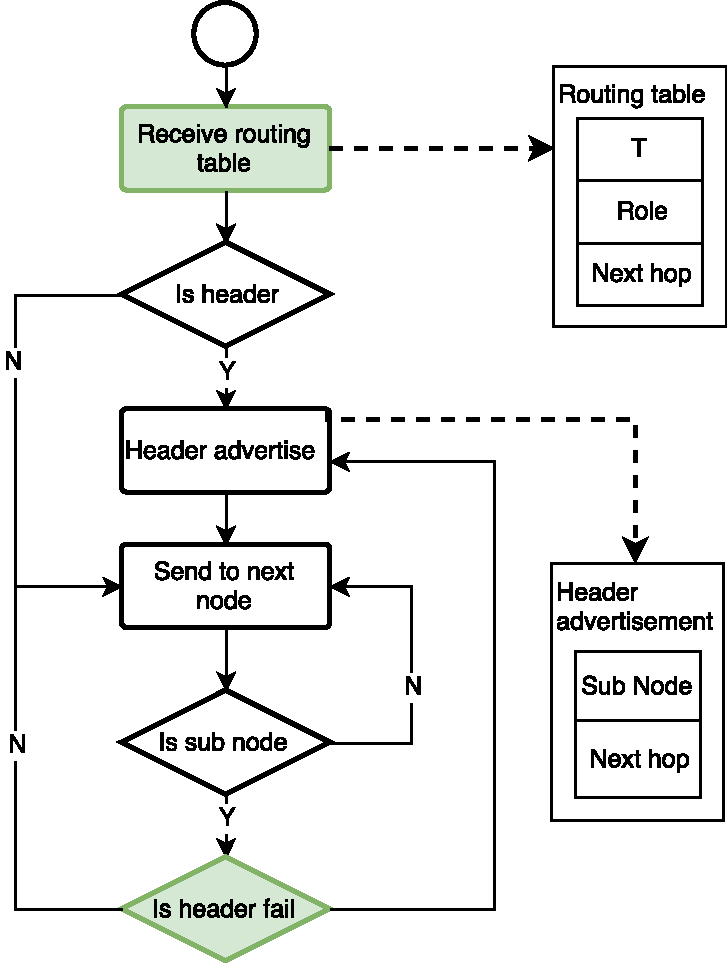
\includegraphics[width=.85\columnwidth]{Figure/routing-flow}
	\vspace{-0.1in}
	\caption{Routing repair}
	\label{routing-flow}
	\vspace{-0.2in}
\end{figure}


\subsection{Network Diagnosis}

\subsubsection{Motivation}

Sensor nodes are provisioned with low-capacity batteries and will run out of energy in the end. 
Besides, uncertain environmental factors will lead to the failure of communications.
Upon these two factors, there occurs network faults such as failure nodes and lossy links from time to time.

Network fault diagnosis is then designed to help network administrators monitor the network 
operational status and maintain a sensor network system. The key idea of the existing works
on fault diagnosis is to collect running information from nodes and deduce root causes of network
exceptions. The running information is collected by a mechanism of probing.

We implement the network diagnosis process as an application in our {\sdn} system.
Since in {\sdn} we have our mobile UAV as a controller, a more flexible way is to infer the suspicious 
nodes of the network fault in traditional way first and then set the UAV to check out the fault sources. 
 
\subsubsection{Design}

We first introduce a state-of-the-art algorithm named DID 
\cite{gong2015directional}, which is a directional diagnosis approach.
We utilize the node tracing module and the tracing collection module of DID
to infer the suspicious nodes in our network diagnosis application, 
and then set our UAV controller to confirm the network elements being faulty.

The node tracing module is conducted in each sensor node. 
Every time a packet arrives at a node, it counts
the source of the packet . The tracing collection module
is set in the UAV controller. When network exception is detected, 
it gathers the tracing information in the tracing module of the relevant nodes
and infers a suspicious node set. Next we set the UAV to fly through the 
node set and check each node first to diagnose the failed nodes. 
Then UAV collects the neighbor lists of all the nodes in the suspicious node set.
With the collected neighbor lists, the UAV controller reconstructs the topical topology and 
compares it with the default topology to find the failed links.

Compared to DID, the diagnosis application in {\sdn} releases the complicated inference
computations and can achieve accurate diagnosis since the UAV can fly to the sensors 
to confirm the network faults. {\sdn} can realize the four types of fault sources the same as DID:  
\begin{itemize}
\item	Node failure. This network failure is caused by the node itself.
\item	Link failure. This network failure is caused by the communication links 
between nodes, mainly relating to traffic flow in networks.
\item	Temporary failure. This  network failure is caused by complex interior or exterior 
interferences and quick self-recovery
\item	Multiple failures. This  network failure is caused by multiple failures above.
\end{itemize}



\subsection{AI Node Selection}

\subsubsection{Motivation}

It is inevitable that there will be a part of redundant sensors when deploying a 
practical wireless sensor network. These redundant nodes have overlaps of
observation regions, and what makes the matter worse is that redundant nodes
may cause great communication interference. Therefore it is significant to select 
proper sensors to avoid data redundancy and save the sensor network energy consumption.

In {\sdn}, we provide the node selection application to users. The SDN controller executes the 
selecting algorithm and send the control instructions to activate the selected nodes.

\subsubsection{Design} Our {\sdn} system provide two main node selecting methods: 
greedy selection algorithm and SRSSS algorithm. This application will be extended to more elegant 
algorithms in our future work. 

\textbf{Greedy selection algorithm.} We first provide a simple method to select 
the redundant nodes by a greedy selection algorithm, as described in Alg. \ref{Greedy}. 
The key idea is to select nodes as less as possible to coverage the whole area
 based on the location and sensing range. 
 
 We implement the greedy selection algorithm in {\sdn}. The evaluations in section \ref{Eva} 
 show it greatly saves the sensors' energy and thus prolongs the network lifetime.

\begin{algorithm}
\caption{Greedy Selection Algorithm}
\label{Greedy}
\begin{algorithmic}[1]
\STATE Input: Sensor set $N$, Selected set $M$, Target area $\Omega$, Covering area $\Phi$;
\STATE Initialize : $M = \emptyset$, $\Phi = \emptyset$
\WHILE {$M \neq N$}
    \IF{$\Phi = \Omega $}
        \STATE break; $\backslash$$\backslash$ Selected set has been found
    \ENDIF
    \IF{$\forall n_i \in (N-M) : range(n_i) \subset \Phi$}
    	 \STATE break;$\backslash$$\backslash$ Cannot cover the target area;
    \ENDIF
    \STATE Find $n_i : argmax(\Phi \cap range(n))$, $n_i \in (N-M)$;
    \STATE $\Phi = \Phi \cup {n_i}$
\ENDWHILE
\STATE Output: $M$;
\end{algorithmic}
\end{algorithm}

\textbf{Spatially regularized streaming sensor selection (SRSSS).} 
To realize more intelligent and effective sensor selection, we introduce 
a state-of-the-art AI algorithm named spatially regularized streaming 
sensor selection (SRSSS) \cite{li2016spatially}.

Different from the greedy selection algorithm, SRSSS is a multi-variate 
interpolation framework and focuses on selecting a subset
of sensors in a streaming scenario to minimize collected information redundancy.  

Traditional wireless sensor network is not suitable to implement an AI selection approach
due to the limited computational capability of sensors. Some work use the database to collect data
and make decisions by multi-hop communications. However, in this way the network will use up a great deal of energy.
In our {\sdn}, the UAV fly through the nodes to pick up the collected data and executes the computations.
Then it sends the control instructions to the nodes by one-hop communication and greatly saves the network energy.

The aim of SRSSS is to optimize its objective function which is an equation given
certain constraints of collected information, location and energy consumption.
The objective function is formulated as:

\begin{equation}
\label{OF}
\begin{aligned}
& (W_{k+1},z_{k+1})  \\
& = arg \min_{W,z} \sum_{i=1}^k \mu^{k-i}\lVert X_k^iD_zW(I-D_z)-X_k^i(I-D_z)\rVert^2_2 \\
& + \alpha\sum_{i,j=1}^n\lVert y_i-y_j\rVert_2\lvert W_{i,j} \rvert - \beta\sum_{i,j=1}^n\lVert y_i-y_j\rVert_2 z_iz_j \\
& + \lambda\lVert W \rVert^2_F \\
&s.t. z = [z_1,...,z_n] \in {\{0,1\}}^n, c^Tz \leq P
\end{aligned}
\end{equation}

The first term in (\ref{OF}) is to minimize the prediction error of the collected data
and the following two terms incorporate spatial information. The last term constrains
the complexity of the learned matrix $W$. The energy constraint is controlled by 
the inequality in (\ref{OF}). Because of the limitation of length,  we leave out all the details. 
The meaning of the parameters and the mechanism of 
SRSSS can be seen in \cite{li2016spatially}. 

With the AI sensor selection process, {\sdn} becomes a smarter and adaptive sensor systems. 




\subsection{AI Energy Prediction}

\subsubsection{Motivation}
Wireless sensor networks (WSN)  generally use multi-hop for data collection,
and due to limited compute capability and storage capacity, sensors are unable
to do data mining. Hence, self optimization is impossible.

The sensor next to data center always has the most routing task, which leads to
the heaviest workload and the shortest battery life. Worse more, after the
first sensor run out of energy, a new sensor will be selected to take the place 
of it with more workload. As a result, its lifetime is shorter and the whole 
sensor network will soon run out of energy. We call this Energy exhausted problem.

An ideal solution for Energy exhausted problem is to find a self-adjust routing schedule which 
according to  Energy status of each sensors. Actually, it is a kind of dynamic programming 
problem, the optimization target is the longgest lifetime of the whole network, with
complex constrains. We modified linear and simple MLP deep learning model to simulate and simplified
this constrains. Challenges occurs in traditional WSN because of lack
of global information energy information. With the help of UAV, our {\sdn} system can do
this optimization


\subsubsection{Design}



\subsection{Multi-tasks}

\subsubsection{Motivation}

Wireless sensor networks (WSN)  generally comprise of a group of 
spatially dispersed sensors. In a wireless sensor network, 
sensor nodes are equipped with various 
types of sensors monitoring and recording 
environmental conditions like temperature, sound, sunlight,
humidity, etc.

A given sensing task involves multiple sensors to 
achieve a certain quality-of-sensing.
Generally, an efficient task scheduling for the nodes is that nodes 
are able to perform multiple tasks simultaneously. 
For example, sensors deployed in a grove are assigned tasks to collect
sunlight, temperature and humidity data and these tasks require different 
number of  nodes with respective sensing range, rate and duration.
However, traditional sensor networks are not suitable to conduct this 
multi-tasks due to the limitations of computation complexity for task 
arrangement of each node.

In our {\sdn} system, we implement the multi-tasks application 
with the help of the central controller. The SDN controller
maintains programmable task scheduling and management
modules while sensor nodes are loaded with interfaces to
receive task control instructions.     

\subsubsection{Design}

A deployed wireless sensor networks are usually assigned  with
different data collection requirement. In {\sdn}, we design and 
implement multi-task application and provide easy-to-use
interfaces to users.

When a user assign a task to {\sdn}, the UAV controller will first check out 
the energy and storage constraints of the required sensor set, as described in Alg. \ref{}. 
If the task requirement exceeds the capacity of the sensor set, it will be sent to a     
task queue; Otherwise it will be put into the task buffer to conduct.


\begin{algorithm}
\caption{Sensor Constraint Detection}
\label{Constraint}
\begin{algorithmic}[1]
\STATE Input: Sensor set $N$, Task $T$;
\STATE Input: Remaining Energy for each node :$Energy(u_i)$;
\STATE Input: Remaining Storage for each node :$Energy(u_i)$;
\STATE Initialize: Energy capacity $\eta$, Storage capacity $\xi$;
\STATE Calculate the energy cost of $T$ for each sensor as : $\phi$;
\STATE Calculate the storage cost of $T$ for each sensor as :$\varphi$;
\FOR{Each node $u_i$ in $N$}
	\IF{$Energy(u_i)+\phi \geq \eta \Vert Storage(u_i)+\varphi \geq \xi$}
   	 \STATE Set $T$ to task queue;
   	 \ENDIF
\ENDFOR
\STATE Set $T$ to task buffer;
\end{algorithmic}
\end{algorithm}


A sensor node may have different sensing ranges for different tasks.


There are several practical requirements.

Different tasks have different requirements, including time, sensing range, sensing ratio, etc.

For example tasks like sunlight collection only need to be carried out during the daytime.

Our system provide a task scheduling to 

Sensors are usually assigned multi-tasks.

Sensors are assigned tasks to monitor a specific area.

\begin{table*}[htbp]
	\caption{Task Buffer}
	\label{TB}
	\centering
	\scalebox{0.9}{
	\begin{tabular}{|l|l|l|l|l|}
		\hline
		Task ID& Node set& Sensing rate & Sensing range& Sensing duration \\
		\hline
		Task ID& Node set& Sensing rate & Sensing range& Sensing duration \\
		\hline
		...& ...& ... & ...& ... \\
		\hline
		Task ID& Node set& Sensing rate & Sensing range& Sensing duration \\
		\hline
		...& ...& ... & ...& ... \\
		\hline
		\end{tabular}
	}
\end{table*}

Different tasks have different requirements, i.e. 

\begin{itemize}
\item \textbf{Node set.} Users can assign tasks to 
\item \textbf{Sensing rate.}
\item \textbf{Sensing range.} The maximum distance that a node can detect. 

\item \textbf{Sensing duration.} The sensing time from start to end. 
There is no need to collect sunlight data at night.
\end{itemize}

Task scheduler do the arrangement. 

Task buffer.

Task queue.

Scheduling table.

...

